\chapter{Implementazione}

\section{Descrizione del progetto}
\label{descrizione_progetto}

% \todo{Una descrizione del progetto, con la separazione in fasi}
Il progetto si pone l'obiettivo di raccogliere una quantità rappresentativa
di paper, autori e conferenze degli ultimi anni al fine di derivare alcune
correlazioni fra le principali metriche, quali l'$h$-index, la qualità delle
conferenze ed il numero delle citazioni.

Il lavoro si suddivide principalmente nelle seguenti fasi:
\begin{enumerate}
  \item Modellazione dei dati inerenti al problema;
  \item Raccolta e organizzazione dei dati da varie fonti, quali Scopus e GGS;
  \item Integrazione dei dati in un unico modello al fine di creare un database unificato;
  \item Sviluppo di un'applicazione web in Django per la visualizzazione delle varie metriche.
\end{enumerate}

Oltre agli indici direttamente disponibili (e.g., $h$-index, citazioni, qualità
delle conferenze), sono state derivate alcune metriche per via campionaria.
Tra le principali analizzate vi sono:
\begin{itemize}
  \item La distribuzione della qualità delle conferenze analizzate;
  \item La distribuzione degli $h$-index degli autori;
  \item La distribuzione della qualità dei lavori per un certo autore;
  \item La correlazione tra qualità delle conferenze e distribuzione del numero delle citazioni dei paper;
  \item La correlazione tra la qualità di una conferenza e la distribuzione degli $h$-index degli autori coinvolti.
\end{itemize}
\todo{Vedere di aggiungerne altre}

%%%% STRUMENTI %%%%%
\section{Strumenti}

I dati che sono stati analizzati in questo progetto di tesi sono stati scaricati
dal database di Scopus utilizzando le API che il sito mette a disposizione.

Per implementare la dashboard e le varie pagine che mostrano i risultati delle
interrogazioni è utilizzato Python come linguaggio di programmazione, il
framework Django e SQLite come database.

%%%% SCOPUS API %%%%%
\subsection{Scopus API}

Scopus permette di accedere a circa 78 milioni di articoli, riviste
scientifiche, libri e pubblicazioni. Le API di Scopus permettono di visualizzare
abstract e dati riguardanti il numero di citazioni di tutte le riviste
accademiche indicizzate da Scopus.

Sono disponibili due modi di utilizzo delle API di Scopus: commerciale e
non commerciale. Per questa tesi sono state utilizzate le API a uso non
commerciale, disponibili gratuitamente per lavori senza scopo di lucro.
Utilizzando le API di Scopus si ha accesso diretto ai dati in tempo
reale. Le \textit{API responses} includono link a risorse collegate, rendendo
la navigazione più semplice e la documentazione consente di visualizzare in
anteprima la richiesta e la risposta della API in modo interattivo. Inoltre
l'architettura RESTful permette di avere vantaggi di scalabilità, portabilità
e affidabilità.
Tali API risultano però sottoposte ad alcuni limiti, in quanto sono accessibili
solo da reti di atenei riconosciute da Scopus ed implementano rate limiting\footnote{\url{https://dev.elsevier.com/api_key_settings.html}}.

Una categoria di API importante è rappresentata dalla \textit{Scopus Search}~\cite{scopussearch}.
Essa può essere usata per accedere a dati riguardanti
paper, con relativi autori ed atenei. Ogni risultato fornito è collegato ad un
abstract e tramite link al resto del testo dell'articolo.
Questa API utilizza la sintassi booleana che consente agli utenti di combinare
parole chiave attraverso gli operatori \texttt{AND}, \texttt{OR} e \texttt{NOT},
per poter produrre risultati  più rilevanti. La ricerca booleana viene inviata
tramite il parametro \textit{query} della \textit{query string} e il contenuto
della ricerca inviata deve essere  codificato nell'URL.

\subsection{pybliometrics}\label{sec:pybliometrics}

\texttt{pybliometrics}~\cite{pybliometrics} è una libreria di Python che serve per estrarre e memorizzare nella cache i dati dal database Scopus.
Essa fornisce un insieme di classi che forniscono un'astrazione dalle chiamate
API di Scopus. Tali classi sono:
\begin{itemize}
	\item \texttt{AbstractRetrieval}: implementa l'API Abstract Retrieval di
	Scopus che consente di estrarre informazioni riguardo gli articoli;
	\item \texttt{AffiliationRetrieval}: implementa l'API Affiliation Retrieval
	di Scopus che fornisce informazioni riguardo gli atenei registrati, come per
	esempio città, paese e membri;
	\item \texttt{AuthorRetrieval}: implementa l'API Author Retrieval di Scopus
	che contiene tutte le informazioni riguardanti un autore;
	\item \texttt{ScopusSearch} implementa l'API di ricerca di Scopus, esegue una
	query per cercare documenti e quindi recupera i record della query.
\end {itemize}

Un esempio d'uso della API, preso da~\cite{pybliometrics}, è dato dal
Listing~\ref{lst:pybliometrics-example}.

\begin{lstlisting}[language=Python, caption=Esempio d'uso di \texttt{pybliometrics}, label=lst:pybliometrics-example]
from pybliometrics.scopus import AbstractRetrieval, AuthorRetrieval, AffiliationRetrieval

ab = AbstractRetrieval("10.1016/j.softx.2019.100263")

print(ab.title) # 'pybliometrics: Scriptable ...'
print(ab.authors) # > [Author(...), Author(...)]

au1 = AuthorRetrieval(ab.authors[0].auid)
au2 = AuthorRetrieval(ab.authors[1].auid)

print(au1.affiliation_current) # [Affiliation(...)]
print(au2.h_index) # 34

aff1 = AffiliationRetrieval(au1.affiliation_current[0].id)

print(aff1.author_count) # 98
\end{lstlisting}

\subsection{matplotlib}

\texttt{matplotlib}~\cite{matplotlib} è una libreria Python per la creazione
di grafi e visualizzazioni di dati in Python. In questo progetto la libreria
è stata usata per la creazione dei grafici rappresentanti metriche aggregate,
come ad esempio la distribuzione delle conferenze secondo il loro rating, 
al fine di semplificare la fruizione dei vari indici.

Inoltre, la libreria permette l'export delle visualizzazioni in vari formati,
come PNG, JPEG e PDF, anche integrabili direttamente in risposte a chiamate HTTP.
Fornisce inoltre la possibilità di creare visualizzazioni interattive, seppur
non usata in questo progetto di tesi.

L'interfaccia esposta da \texttt{matplotlib} è stata creata appositamente per
essere utilizzabile anche da persone con esperienza pregressa del linguaggio
Matlab, in quanto è molto simile al parco di funzioni fornite da quest'ultimo
per la creazione di grafi. Non solo, anche lo stile grafico predefinito è
ispirato da quello dato da Matlab.

Nel Listing~\ref{lst:matplotlib-example} si può vedere un esempio d'uso per
la creazione di un grafico a barre.

\begin{lstlisting}[float, language=Python, caption=Esempio d'uso di \texttt{matplotlib}, label=lst:matplotlib-example]
import matplotlib.pyplot as plt

xs = ['A++', 'A+', ...]
ys = [10, 20, ...]

plt.figure()
plt.title('Distribuzione del rating delle conferenze')
plt.bar(xs, ys)
plt.xlabel('Rating della conferenza')
plt.ylabel('Numero conferenze')
plt.show()
\end{lstlisting}


%%%% DJANGO %%%%%
\subsection{Django}\label{sec:django}

Django~\cite{django} è un framework web open source scritto in Python. È
un framework ``batteries included'', ovvero tenta di fornire più strumenti
possibile per ridurre sia la quantità di codice da scrivere sia la sua
complessità.

Django si basa sull'architettura \textit{Model, View, Template}, basata sulla più
classica MVC. Essa propone tre diverse entità per la gestione dei dati e dell'interazione
con l'utente, che sono:
\begin{itemize}
	\item \textit{Model}, la descrizione dei dati tramite una classe Python;
	\item \textit{View}, un sistema che processa le richieste degli utenti e
	definisce che dati devono essere presentati in risposta;
	\item \textit{Template}, un template HTML con un proprio linguaggio di templating
	chiamato DTL (Django Template Language) che definisce la rappresentazione
	grafica dei dati.
\end{itemize}
In questa categorizzazione, la \textit{View} di MVT corrisponde al \textit{Controller}
di MVC, mentre il \textit{Template} di MVT corrisponde alla \textit{View} di MVC.

\begin{lstlisting}[language=Python, caption=La classe \texttt{Author}, label=lst:author]
from django.db import models

class Author(models.Model):
    surname = models.CharField(max_length=200)
    name = models.CharField(max_length=200)
    citation_count = models.IntegerField()
    cited_by_count = models.IntegerField()
    h_index = models.IntegerField()
\end{lstlisting}

Django fornisce un ORM (\textit{Object-Relational Mapping}) tramite la
rappresentazione di tabelle con delle classi che derivano dalla classe
predefinita \texttt{Model}, come mostrato nel Listing~\ref{lst:author}. In
tal modo, è possibile interagire con degli oggetti Python, del tutto simili
alle classi, astraendo completamente dalla tecnologia di database utilizzata.
Infatti, con Django è possibile utilizzare diversi DBMS~\cite{djangoDBMS}, tra cui PostgreSQL,
MariaDB, MySQL e SQLite. Quest'ultimo è stato scelto per essere usato in questo
progetto di tesi, in quanto la semplicità e la facilità di setup sono risultate
fondamentali per velocizzare la realizzazione di prototipi.

Le \textit{View} di Django possono essere rappresentate da varie entità nel codice,
ma i modi principali sono le \textit{view generiche} tramite classi fornite dal framework
stesso e delle semplici \textit{funzioni} che lavorano su un parametro rappresentante
la richiesta effettuata dall'utente. Come esempio, nel Listing~\ref{lst:view-author-info}
è rappresentata una view che ottiene le informazioni di un autore specifico,
come salvate su database, aggiungendo inoltre una classificazione in base al
rating delle conferenze a cui ha partecipato.

\begin{lstlisting}[language=Python,caption=La view \texttt{author\_info},label=lst:view-author-info]
def author_info(request, author_id):
    author = get_object_or_404(Author, pk=author_id)
    num_confs = {}

    for pub in author.publication_set.all():
        rating = pub.paper.conference.ggs_rating
        if rating in num_confs:
            num_confs[rating] += 1
        else:
            num_confs[rating] = 1

    return render(request,
                  "author_info.html",
                  {"author": author, "num_confs": num_confs})
\end{lstlisting}

Infine, un \textit{Template} di Django è semplicemente un file HTML che
viene interpretato come codice DTL al momento della costruzione della risposta
inviata dal server al client che ha effettuato la richiesta. Un esempio di tale
template è visibile nel Listing~\ref{lst:django-template}.

\begin{lstlisting}[language=HTML, caption=Template per l'elenco delle conferenze,label=lst:django-template]



Conferences - Produzione Scientifica



<h1>Conferences</h1>

<div class="info" style="flex-wrap: wrap;">
  <div class="info-img">
    <img src="" />
    <span>Distribuzione delle conferenze</span>
  </div>
  
  <div class="info-img">
    <img src="" />
    <span>Distribuzione citazioni per rating</span>
  </div>
  
  <div class="info-img">
    <img src="" />
    <span>Distribuzione citazioni di paper d'impatto per rating</span>
  </div>

  <div class="info-img">
    <img src="" />
    <span>Distribuzione h-index per rating</span>
  </div>

  <div class="info-img">
    <img src="" />
    <span>Distribuzione h-index top conferences</span>
  </div>
  
</div>

<h1>List of Conferences</h1>

<table>
  <thead>
    <tr>
      <th>Name</th>
      <th>Acronym</th>
      <th>Rating</th>
    </tr>
  </thead>
  <tbody>
    
    <tr>
      <td>
      <a href="">{{ conference.name }}</a>
      </td>
      <td>{{ conference.acronym }}</td>
      <td>{{ conference.ggs_rating }}</td>
    </tr>
    
  </tbody>
</table>

\end{lstlisting}

Django offre anche la possibilità di avere più di una \textit{app} su uno stesso
server web, ciascuna con le proprie views, i propri template ed il proprio
database. In questo modo, è possibile separare la configurazione generica del
server gestito da Django da varie applicazioni che girano su di esso.
Per questo progetto, la creazione di una singola app è più che sufficiente.

Django associa ad ogni possibile \textit{path} (o URL) di una richiesta HTTP
una certa view. Quando una richiesta HTTP viene inviata dal client verso il
server gestito da Django, quest'ultimo effettua una ricerca fra i propri path
definiti ed inoltra la richiesta, trasformata in un oggetto Python, alla
\textit{view} che si occupa della sua gestione.
Tale view può eseguire qualsiasi azione desiderata, come aggiorare il database o
leggere dati, anche differenziando in base al metodo HTTP usato dalla richiesta.
Una volta terminato il lavoro necessario, però, la view è costretta a ritornare
una risposta al client, sia essa positiva o negativa, che la mostrerà all'utente
tramite un browser o qualsiasi altro tool usato.

\section{Ottenimento dei dati}

Come già anticipato in Sezione~\ref{sec:scopus}, la maggior parte dei dati è
stata presa da Scopus. In particolare, Scopus ha fornito i dati di circa 80000
papers negli ultimi 4 anni, con i relativi autori ed affiliazioni.
Per le conferenze, non fornendo Scopus informazioni se non nome ed acronimo
delle conferenze, si è fatto uso dei dati indicizzati da GII-GRIN-SCIE~\cite{giigrinscie} (GGS).

Per il download dei dati da Scopus, si è usato \texttt{pybliometrics}
(Sezione~\ref{sec:pybliometrics}) per lo sviluppo di script custom orientati
al download di grandi quantità di dati in modo automatico facendo uso delle
API fornite da Scopus.

Per quanto riguarda le conferenze, invece, i nomi forniti da
GGS non concordano in pieno con quelli presenti su Scopus. A questo fine,
si è manualmente proceduto all'analisi delle conferenze ottenute ed al loro
inserimento all'interno del database del progetto.
Al fine di semplificare e velocizzare il processo, si è fatto uso della
\textit{distanza di Levenshtein} per confrontare i nomi dati dalle due fonti.
La priorità è stata comunque data agli acronimi rispetto ai nomi interi.

\subsection{Distanza di Levenshtein}

L'algoritmo di Levenshtein, introdotto per la prima volta nel
1965~\cite{levenshtein1966} calcola la somiglianza tra due stringhe diverse.
Date due stringhe $a$ e $b$, l'algoritmo misura il numero di modifiche
elementari necessarie per trasformare la stringa $a$ nella stringa $b$.
Tra le operazioni elementari si hanno: eliminazione di un carattere,
sostituzione di un carattere con un altro, inserimento di un nuovo carattere.
Più precisamente, definite $a$ e $b$ due stringhe, $|a|$ la lunghezza di una
stringa, la distanza di Levenshtein è definita come
\begin{equation*}
  \text{lev}(a, b) =
  \begin{cases}
    |a| & \text{se } |b| = 0 \\
    |b| & \text{se } |a| = 0 \\
    \text{lev}(\text{tail}(a), b) & \text{se } a_0 = b_0 \\
    1 + \min\begin{cases}
      \text{lev}(\text{tail}(a), b) \\
      \text{lev}(a, \text{tail}(b)) \\
      \text{lev}(\text{tail}(a), \text{tail}(b)) \\
    \end{cases}
    & \text{altrimenti}
  \end{cases}
\end{equation*}
%
Dove $\text{tail}$ rappresenta la coda di una lista, i.e., se $a_i$ è il
carattere in posizione $i$, allora data la stringa $a = a_0a_1\cdots a_n$ si ha
che $\text{tail}(a) = a_1\cdots a_n$.
Nell'implementazione è stata usata la libreria
\texttt{python-Levenshtein}~\cite{pythonLevenshtein}.

Al fine di dimostrare brevemente il ragionamento intrapreso, si prendano come
esempio le due stringhe \texttt{kitten} e \texttt{sitting}. In tal caso, si
ha che $\text{lev}(\text{kitten}, \texttt{sitting}) = 3$. Infatti, la seconda
stringa si può ottenere dalla prima effettuando le sostituzioni $k \to s$
e $e \to i$, con l'aggiunta finale della lettera \textit{g}.
Di conseguenza, essendo le modifiche elementari pari in numero a 3, esso è
anche il valore assunto dalla distanza di Levenshtein.

%%% DOWNOLAD DEI DATI %%%%
\section{Descrizione dei dati}\label{sec:descrizionedati}

In Figura \ref{fig:logico} è visibile lo schema logico, rappresentante
le tabelle presenti direttamente nel database, coi relativi attributi e chiavi
esterne. Notare la presenza della tabella \textit{Publication}, in sostituzione
alla relazione tripla nominata in Sezione~\ref{sec:modellizzazioni}.

Al fine di identificare univocamente i dati, si è fatto uso dei campi
identificativi forniti direttamente dal database di Scopus. Questo per evitare
ambiguità con un'eventuale generazione automatica a partire dai dati,
soprattutto in caso di omonimie.

\begin{figure}
  \centering
  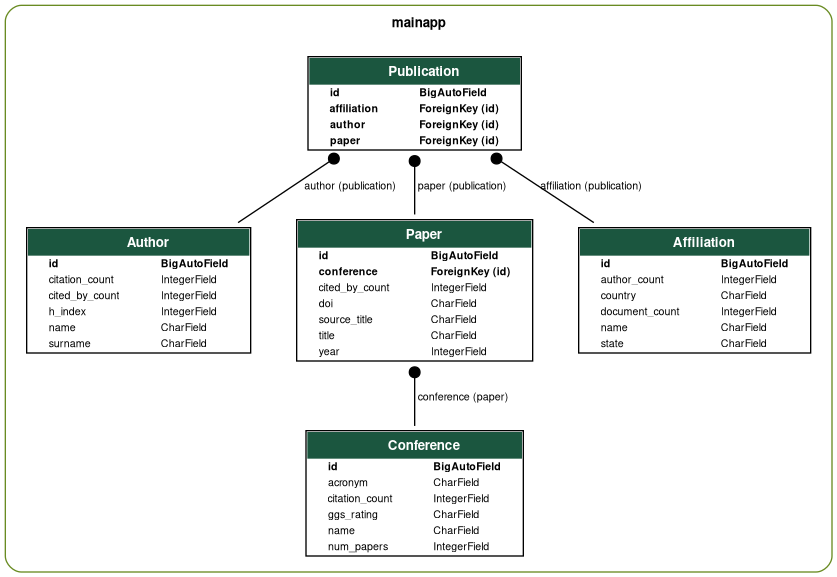
\includegraphics[width=0.8\linewidth]{logico.png}
  \caption{Schema logico del problema}
  \label{fig:logico}
\end{figure}

\subsection{Affiliation}

Un'affiliazione rappresenta un'università, e per ogni singola entry si ha
interesse a mantenere i seguenti campi:

\begin{itemize}
  \item \texttt{aff\_id}, l'identificativo dell'università;
  \item \texttt{affiliation\_name}, nome dell'università;
  \item \texttt{state} e \texttt{country}, contenenti informazioni riguardanti la posizione geografica dell'università;
  \item \texttt{author\_count}, numero di autori associati all'università;
  \item \texttt{document\_count}, numero di documenti per l'università.
\end{itemize}

\subsection{Author}
Un autore è rappresentato dai seguenti campi:
\begin{itemize}
  \item \texttt{author\_id};
  \item dati per il nominativo, ovvero \texttt{surname} e \texttt{name};
  \item \texttt{citation\_count}, numero totale di elementi citati;
  \item \texttt{cited\_by\_count}, numero totale di autori citanti;
  \item \texttt{h\_index}, h-index dell'autore.
\end{itemize}

\subsection{Conference}

Di una conferenza ci interessa mantenere i seguenti campi:
\begin{itemize}
  \item \texttt{title}, nome della conferenza;
  \item \texttt{acronym};
  \item \texttt{ggs\_rating}, il rate come definito da GGS;
  \item \texttt{num\_papers}, numero di paper accettati dalla conferenza;
  \item \texttt{citation\_count}, numero di citazioni totali di tutti i paper della conferenza.
\end{itemize}

\subsection{Paper}

Un paper viene rappresentato dai seguenti dati:

\begin{itemize}
  \item \texttt{id};
  \item \texttt{authors}, lista di autori del paper (rappresentati dai relativi identificativi);
  \item \texttt{title};
  \item \texttt{year};
  \item \texttt{conference}, la conferenza a cui è stato presentato;
  \item \texttt{cited\_by\_count}, il numero di citazioni;
  \item \texttt{doi}, il suo identificativo DOI.
\end{itemize}

% \section{Implementazione di views e metriche}

\section{Applicazione web}

L'applicazione web realizzata in questo progetto di tesi offre la funzionalità
di accesso semplificato ai dati ottenuti e la visualizzazione
delle varie analisi metriche ottenute.

\subsection{Struttura dei file}

% \todo{Descrivere la separazione data da Django nei file e nel codice}

La struttura di file e directory di un'applicazione web scritta con Django 
segue una forma fissa, definita dal framework, che permette l'organizzazione
delle varie parti di codice in base al loro ruolo all'interno dell'architettura.
Le principali sezioni in questo progetto sono date da:
\begin{itemize}
  \item La directory \texttt{mainapp}, che contiene il codice della \textit{app}
        principale di Django;
  \item Il file \texttt{manage.py}, che offre un'interfaccia da riga di comando
        per la gestione di migrazioni sul database, l'avvio e l'arresto di server
        web locali, e simili operazioni di gestione del progetto;
  \item Una directory \texttt{prodsc} per i file usati da Django nella configurazione
        dell'intera applicazione web.
\end{itemize}

A sua volta, la cartella \texttt{mainapp} contiene i seguenti:
\begin{itemize}
  \item \texttt{admin.py}, che contiene le definizioni base per permettere l'uso
        della console di amministrazione offerta da Django;
  \item \texttt{apps.py}, per la configurazione di eventuali app interne a \texttt{mainapp};
  \item \texttt{forms.py}, la definizione del form di upload dei dati, usato per la
        semplificazione della conversione dei dati CSV ottenuti dalle API per
        poter essere inseriti in database;
  \item \texttt{images.py}, che definisce tutte le view per la generazione di
        grafici di metriche tramite \texttt{matplotlib};
  \item \texttt{migrations}, una cartella per le varie migrazioni del database SQLite;
  \item \texttt{models.py}, il modulo che definisce le varie classi dei modelli
        come descritto in Sezione~\ref{sec:django};
  \item \texttt{static}, per file statici come CSS e JavaScript;
  \item \texttt{templates}, directory contenente i diversi template usati dalle view;
  \item \texttt{urls.py}, che definisce gli endpoint accettati da Django e quale
        view è responsabile per la gestione di ciascuno di essi;
  \item Ed infine \texttt{views.py}, le diverse views per la visualizzazione
        dei vari dati utilizzati.
\end{itemize}




%% Dashboard

\subsection{Dashboard}
Di seguito è descritta come è stata realizzata la dashboard per la visualizzazione dei dati e delle metriche realizzate.

Come stile delle pagine web viene utilizzato \textit{Bootstrap}, un framework per lo sviluppo front-end. 
Nel file \texttt{base.html}, contenuto nella directory \texttt{templates}, è contenuto il codice dello stile, che presenta una barra laterale per la navigazione del sito.

In Django si utilizza il tag \texttt{\{\% block \%\}} per definire un blocco che può essere sovrascritto dai modelli che ne derivano. I blocchi utilizzati sono:

\begin{itemize}
  \item \texttt{\{\% block title \%\}}: per il titolo della pagina web;
  \item \texttt{\{\% url \%}\}: per l'url della pagina collegata;
  \item \texttt{\{\% block content \%}\}: per il contenuto della pagina.
\end{itemize}

Nella Figura~\ref{fig:homepage} è mostrata l'hompage del sito che contiene una panoramica generale dell'applicazione e di ciò che consente di visualizzare.

Nella barra di sinistra è possibile andare a visitare le pagine che mostrano più nel dettaglio i dati riguardanti conferenze, autori e affiliazioni. Queste verranno descritte più approfonditamente nelle sezioni successive.

Nella dashboard vengono mostrati i quattro principali grafici estrapolati dall'analisi dei dati: i grafici posti in alto alla pagina mostrano la distribuzione delle conferenze in base al reting e degli $h$-index dei paper; i grafici posti in basso invece mostrano la produttività per nazione in base all'affiliazione e gli $h$-index degli autori per dimensione dell'affiliazione.

\begin{figure}
  \centering
  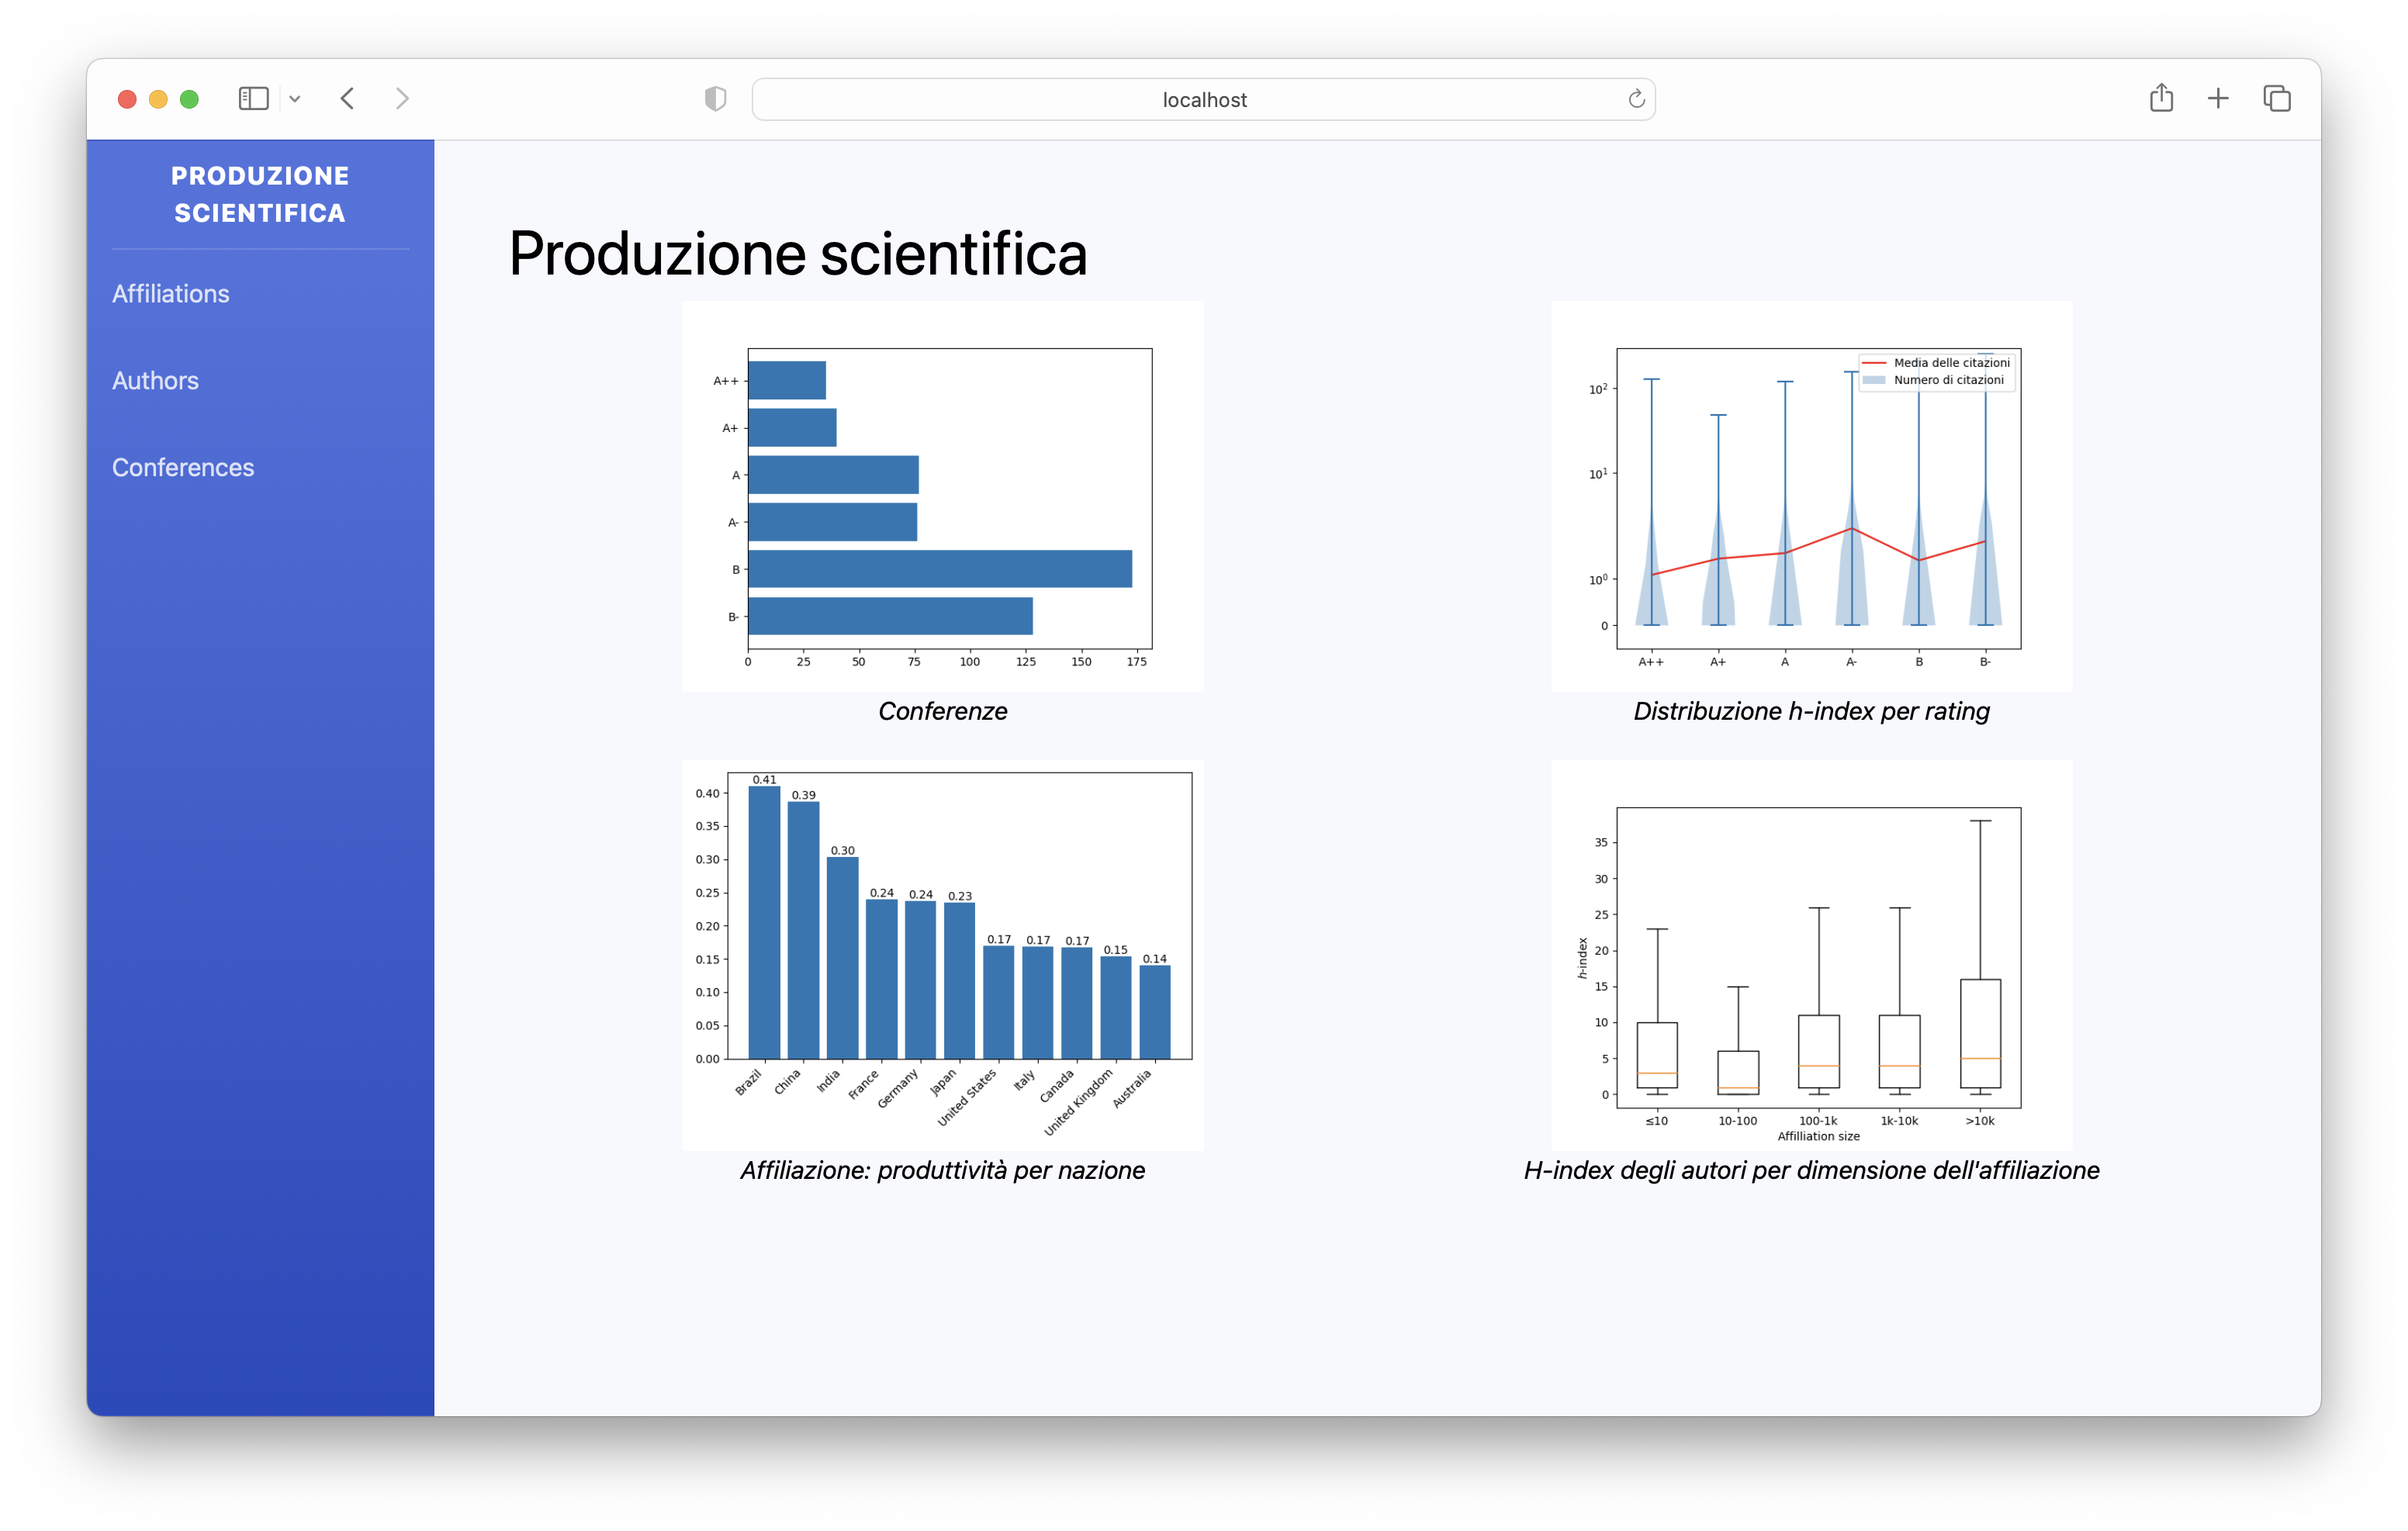
\includegraphics[width=0.8\linewidth]{homepage.png}
  \caption{Homepage della dashboard}
  \label{fig:homepage}
\end{figure}

\subsection{Conferenze}
In questa pagina sono visibili tutte le informazioni relative alle conferenze, come visibile in Figura~\ref{fig:conferences}.
Sono visibili i grafici riguardanti:
\begin{itemize}
  \item La distribuzione delle conferenze in base ai principali rating;
  \item La distribuzione del numero di citazioni del paper in base ai principali rating;
  \item La distribuzione del numero di citazioni di paper di impatto in base ai principali rating;
  \item La distribuzione dell'$h$-index di un autore in base ai principali rating;
  \item Distribuzione degli $h$-index di un autore per le top conferences di sicurezza.
\end{itemize}

\begin{figure}
  \centering
  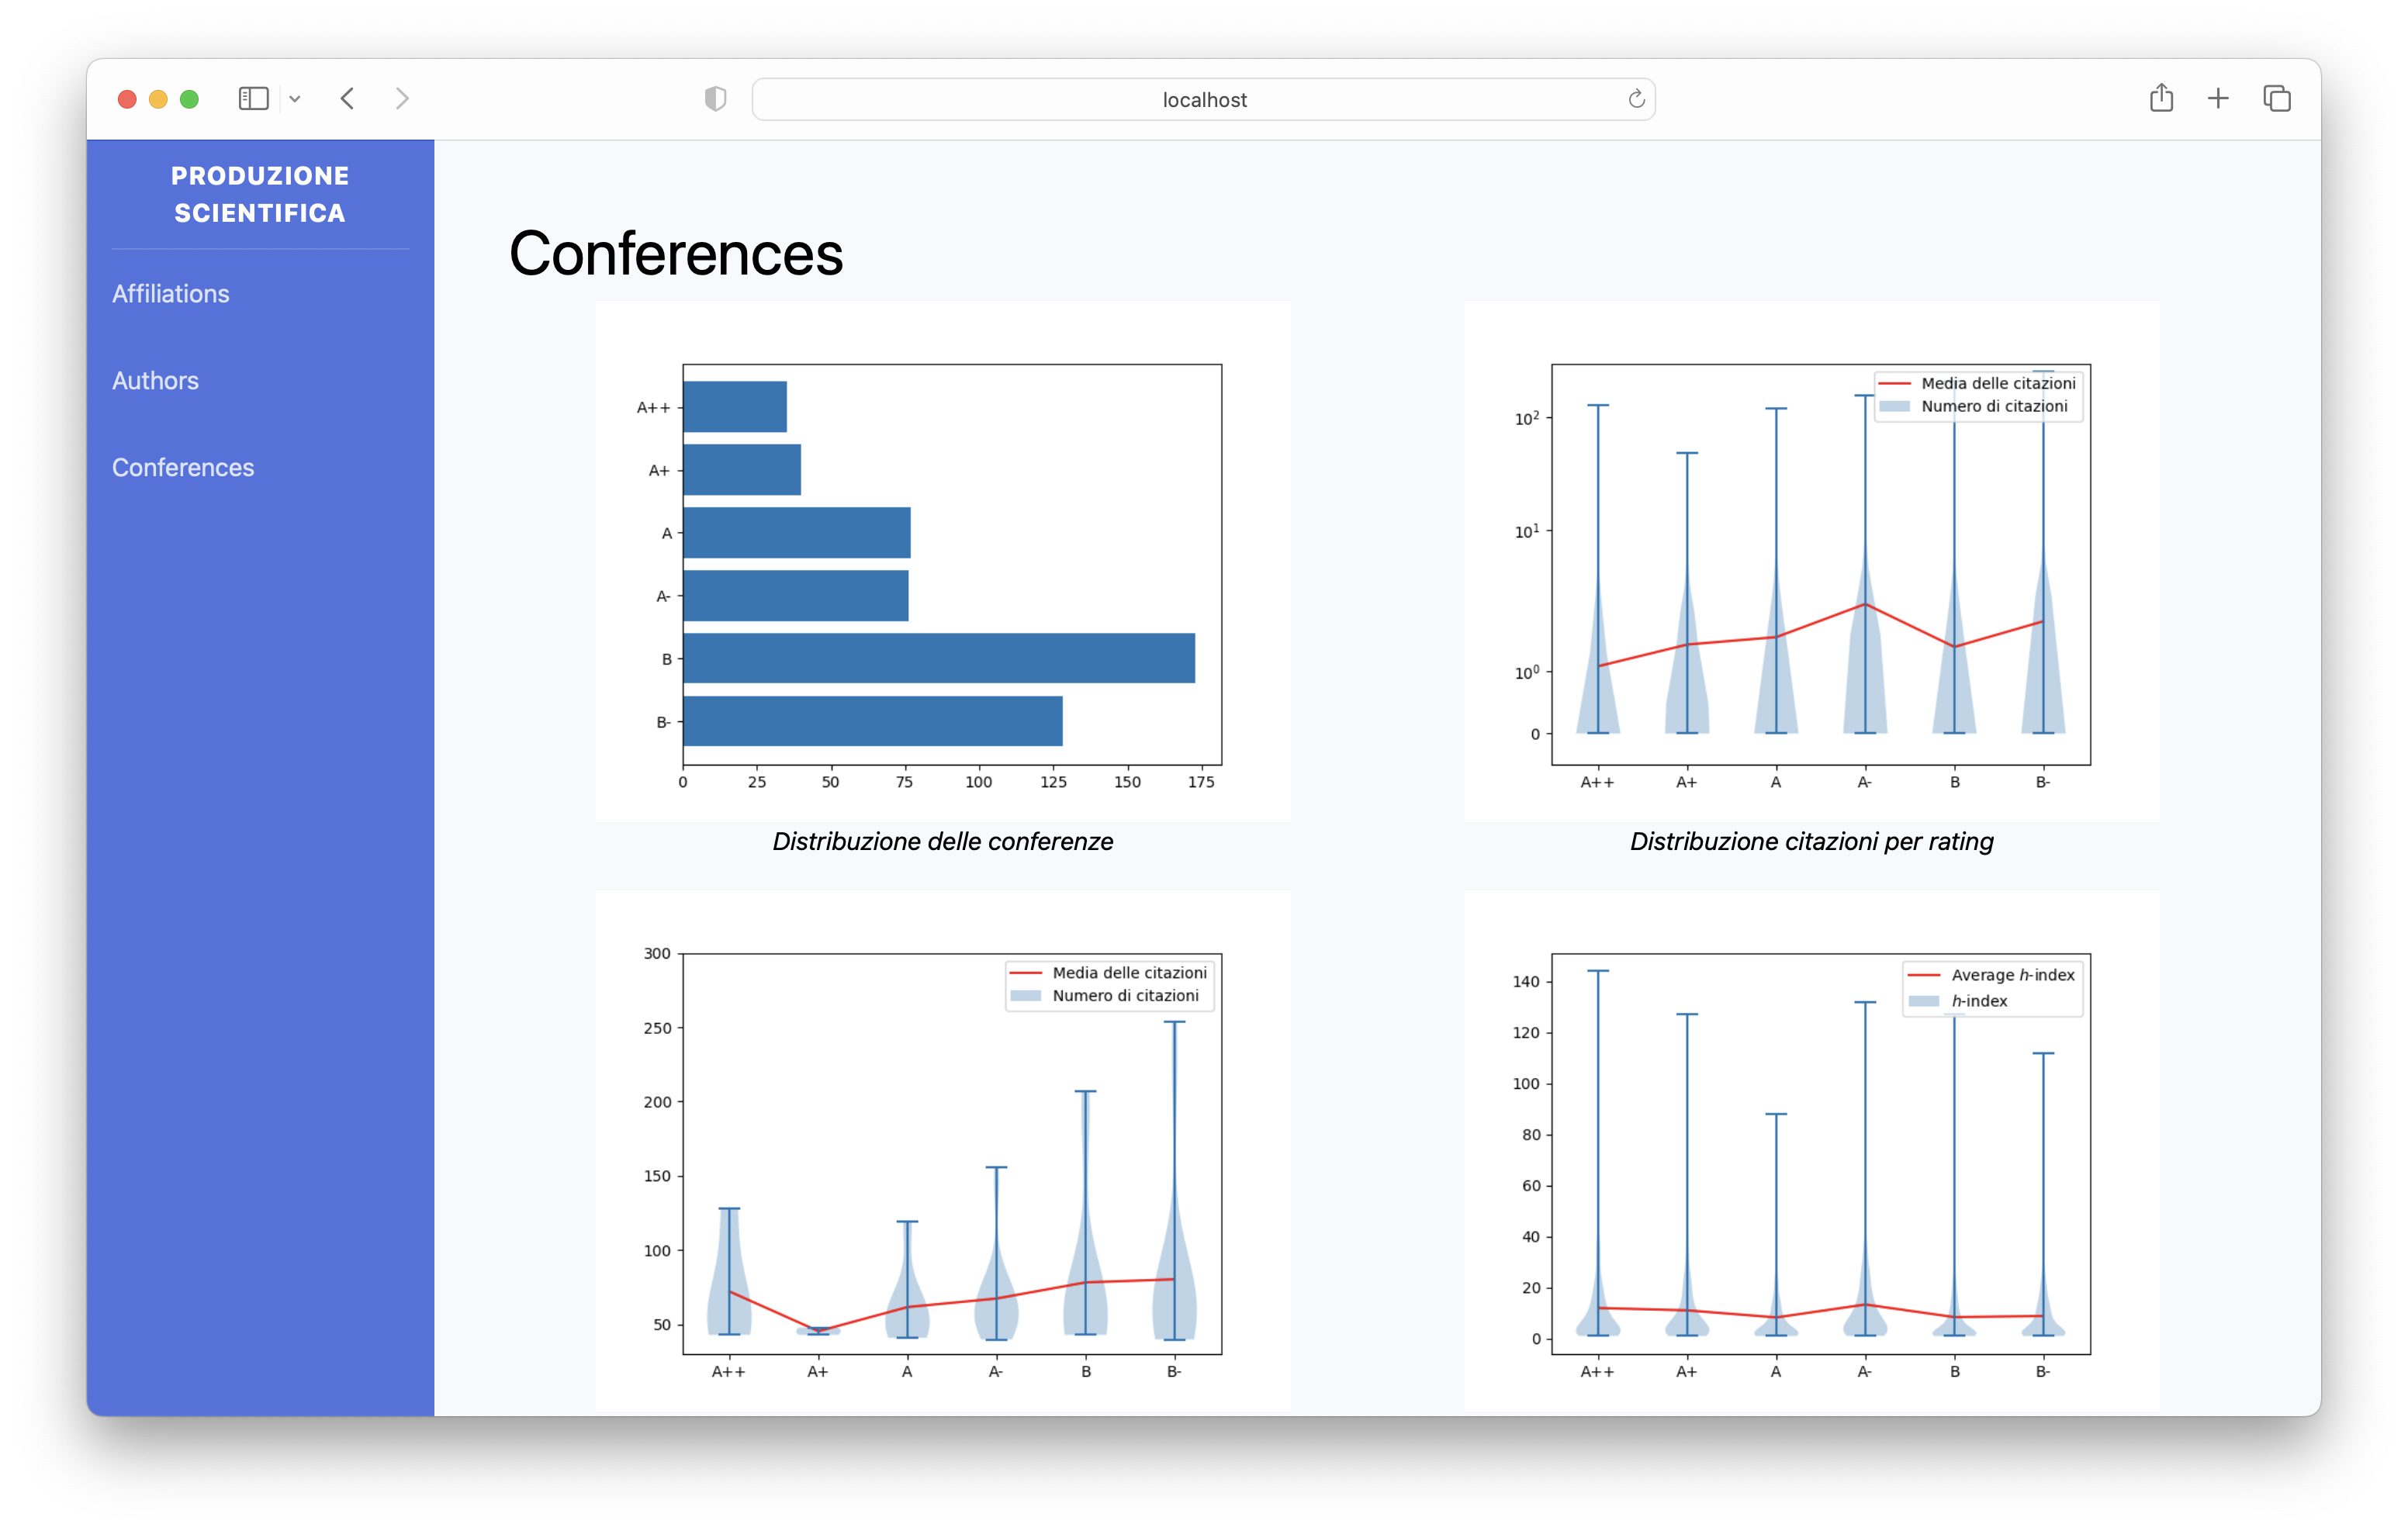
\includegraphics[width=0.8\linewidth]{conferences.png}
  \caption{Pagina delle conferenze}
  \label{fig:conferences}
\end{figure}


Inoltre, nella stessa pagina, è possibile consultare l'elenco delle conferenze con il rispettivo acronimo e rating, come visibile in Figura~\ref{fig:list-conferences}. Nel Listing~\ref{lst:django-template} è mostrato il codice della pagina.


\begin{figure}
  \centering
  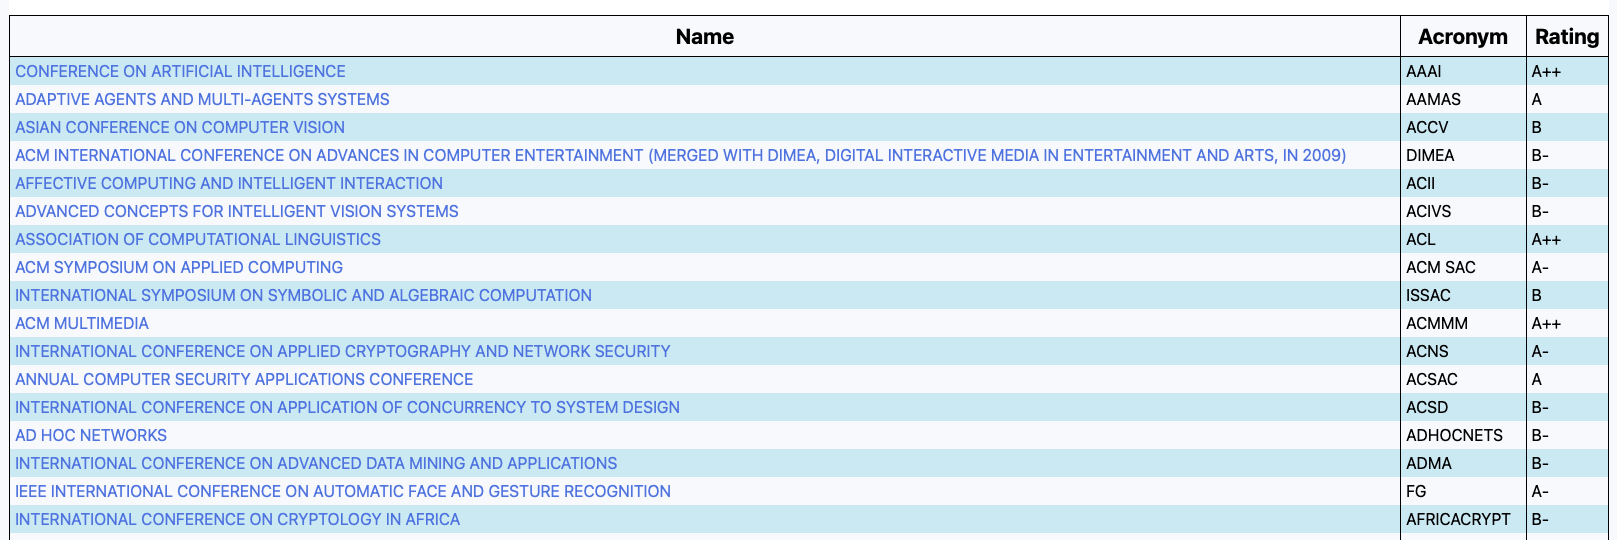
\includegraphics[width=0.8\linewidth]{listConferences.png}
  \caption{Pagina per la visualizzazione della lista delle conferenze}
  \label{fig:list-conferences}
\end{figure}

\subsection{Autori}
Nella pagina sono disponibili le informazioni relative agli autori e le metriche che sono state analizzate.

Come fatto per le conferenze, anche per gli autori sono disponibili i grafici delle metriche che li riguardano e una lista che mostra l'id dell'autore e il nome, come visibile in Figura~\ref{lista-autori}. I grafici consultabili sono:
\begin{itemize}
  \item Numero di citazioni dell'autore in base alla grandezza delle affiliazioni;
  \item $H$-index dell'autore per grandezza dell'affiliazione.
\end{itemize}

Per ogni autore poi è possibile visualizzare i suoi dati, come il numero di citazioni e l'$h$-index. Inoltre viene mostrata anche la distribuzione delle conferenze a cui ha partecipato, calcolata come visibile nel Listing~\ref{lst:distribuzione-autore}.

\begin{lstlisting}[language=html, caption=Estratto di \texttt{template/author\_info.html per la visualizzazione della distribuzione delle conferenze a cui l'autore partecipa}, label=lst:distribuzione-autore]
  <h2> Distribuzione conferenze </h2>
  <ul>
  
  <li>{{ rating }}: {{ count }}</li>
  
  </ul>  

\end{lstlisting}

\begin{figure}
  \centering
  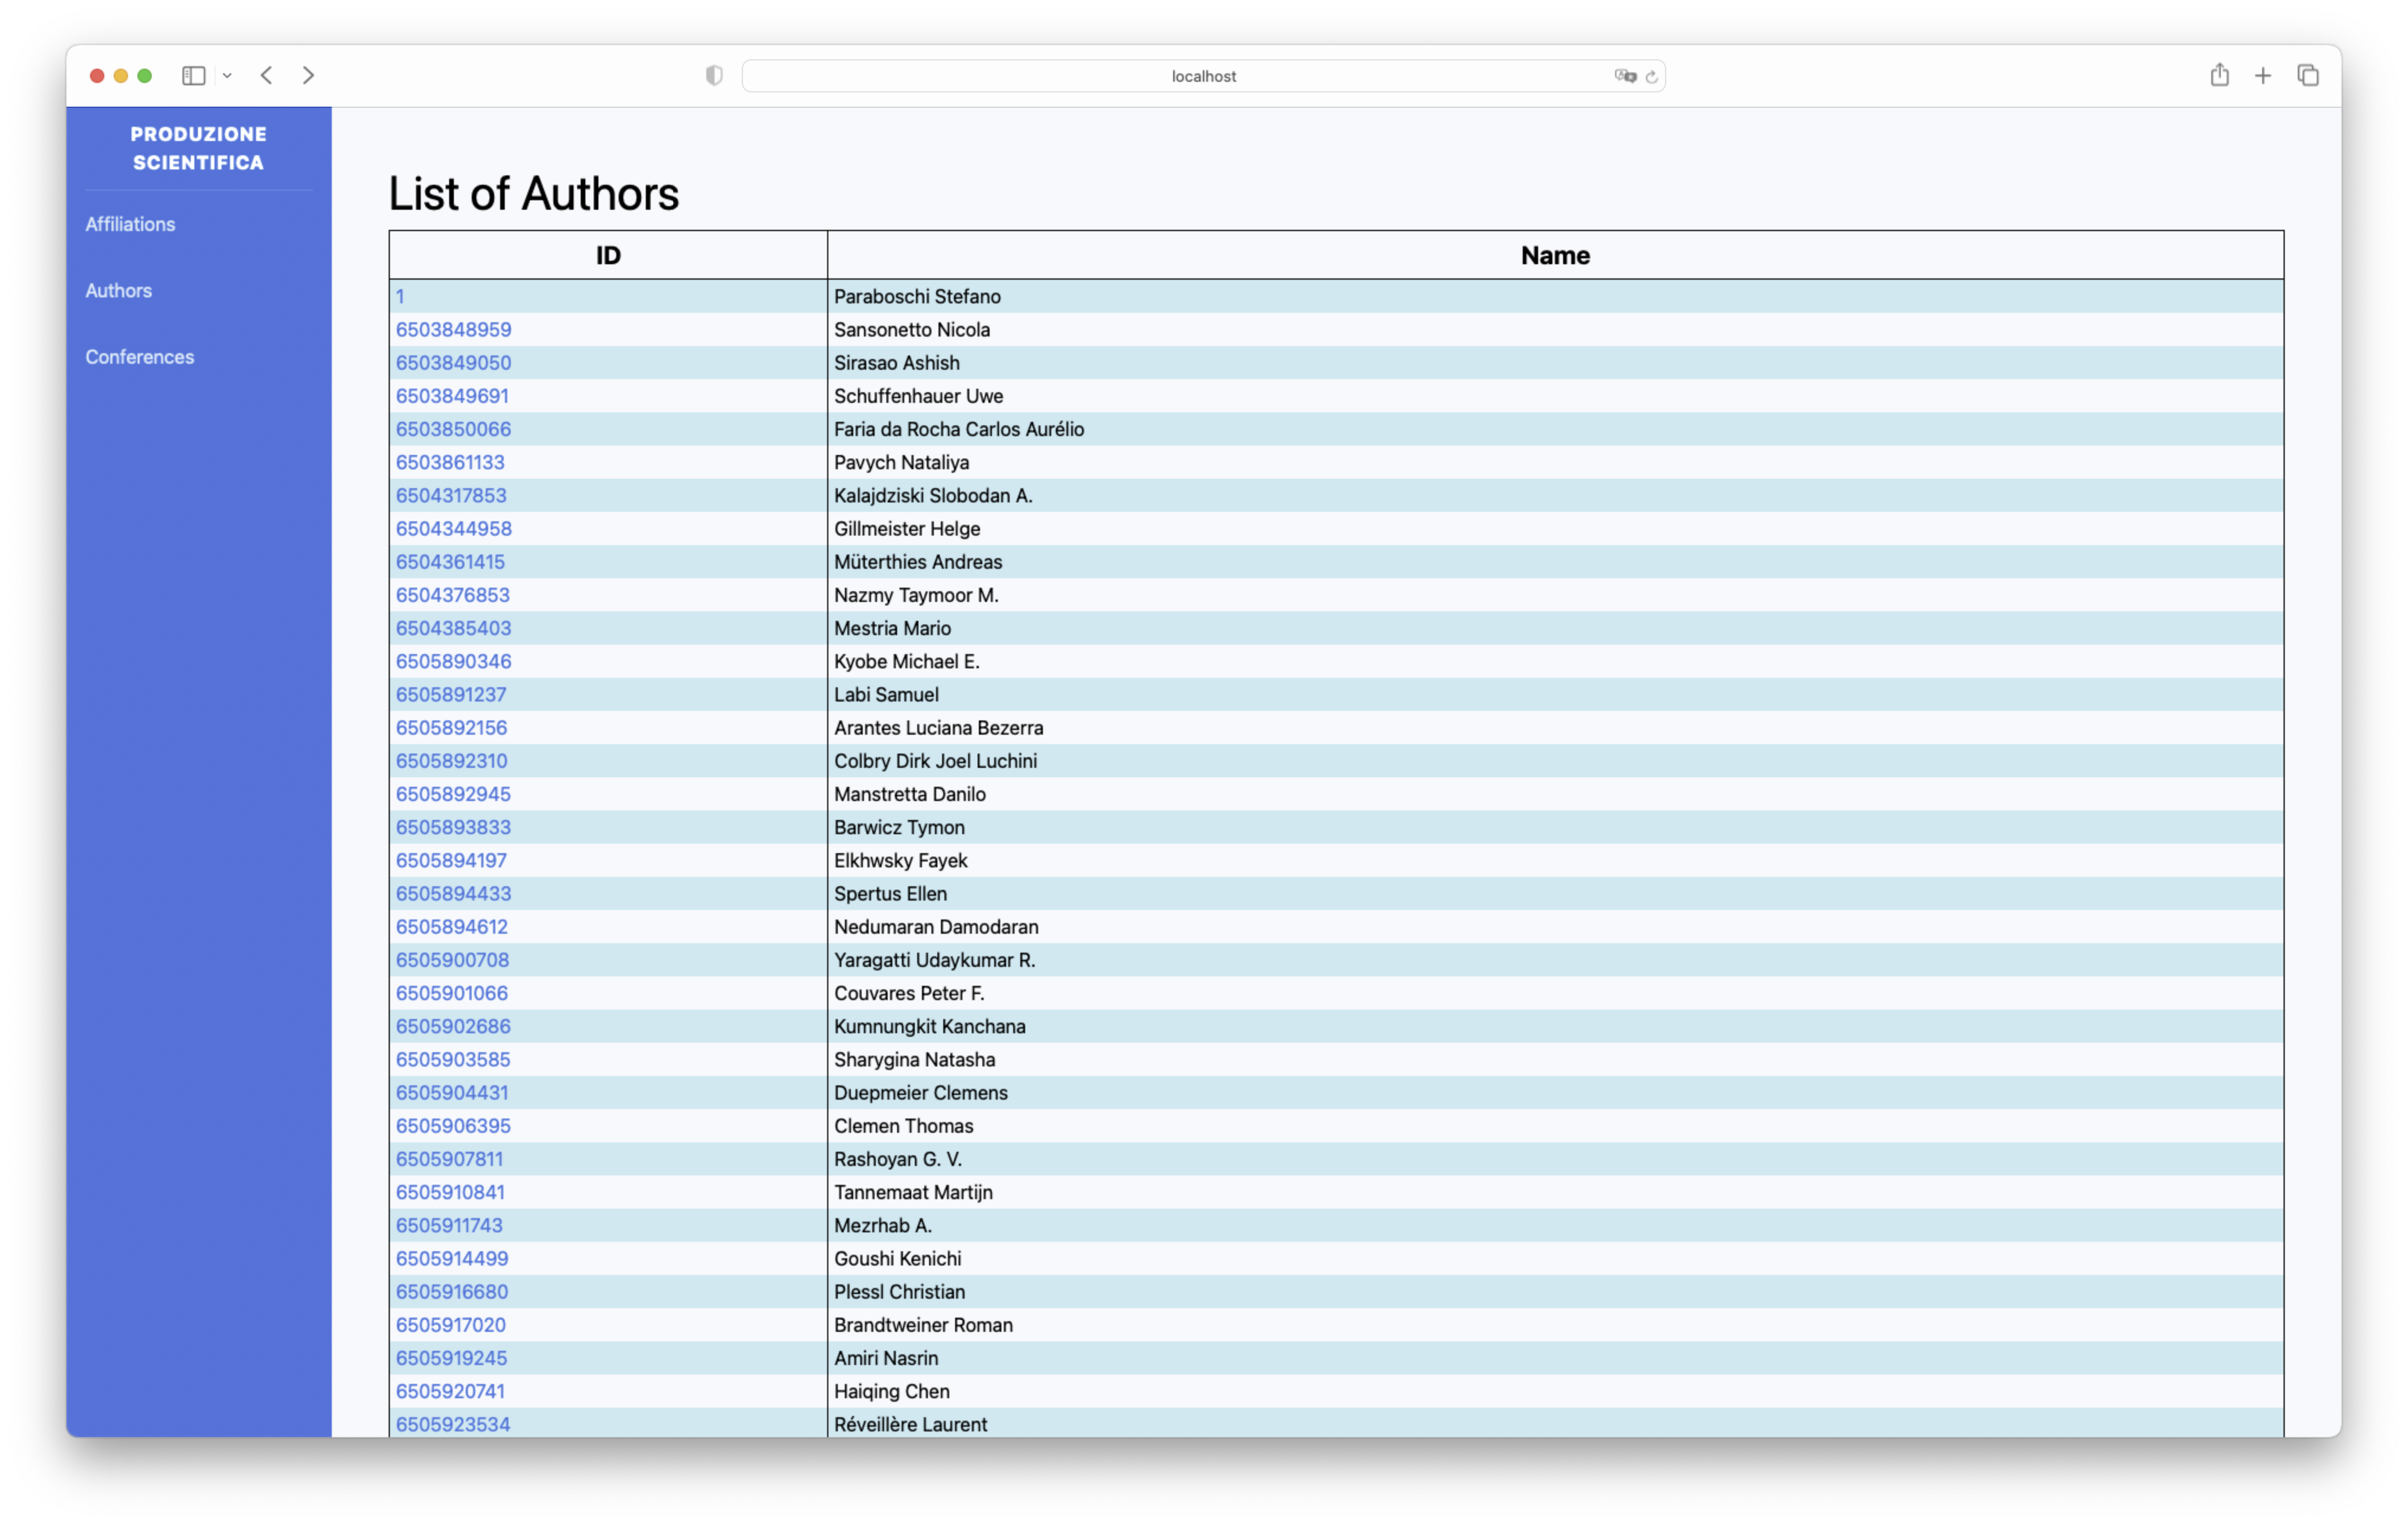
\includegraphics[width=0.8\linewidth]{author_list.png}
  \caption{Pagina degli autori}
  \label{fig:lista-autori}
\end{figure}



\subsection{Affiliazioni}

Nella pagina sono disponibili le informazioni relative alle affiliazioni e le metriche che sono state analizzate.

Come prima, anche per le affiliazioni sono disponibili i grafici delle metriche che li riguardano e una lista per visualizzarne l'elenco, come visibile in Figura~\ref{fig:affiliations}. I grafici consultabili sono:
\begin{itemize}
  \item Numero di autori per nazione;
  \item Numero di documenti per nazione;
  \item Produttività per nazione.
\end{itemize}

\begin{figure}
  \centering
  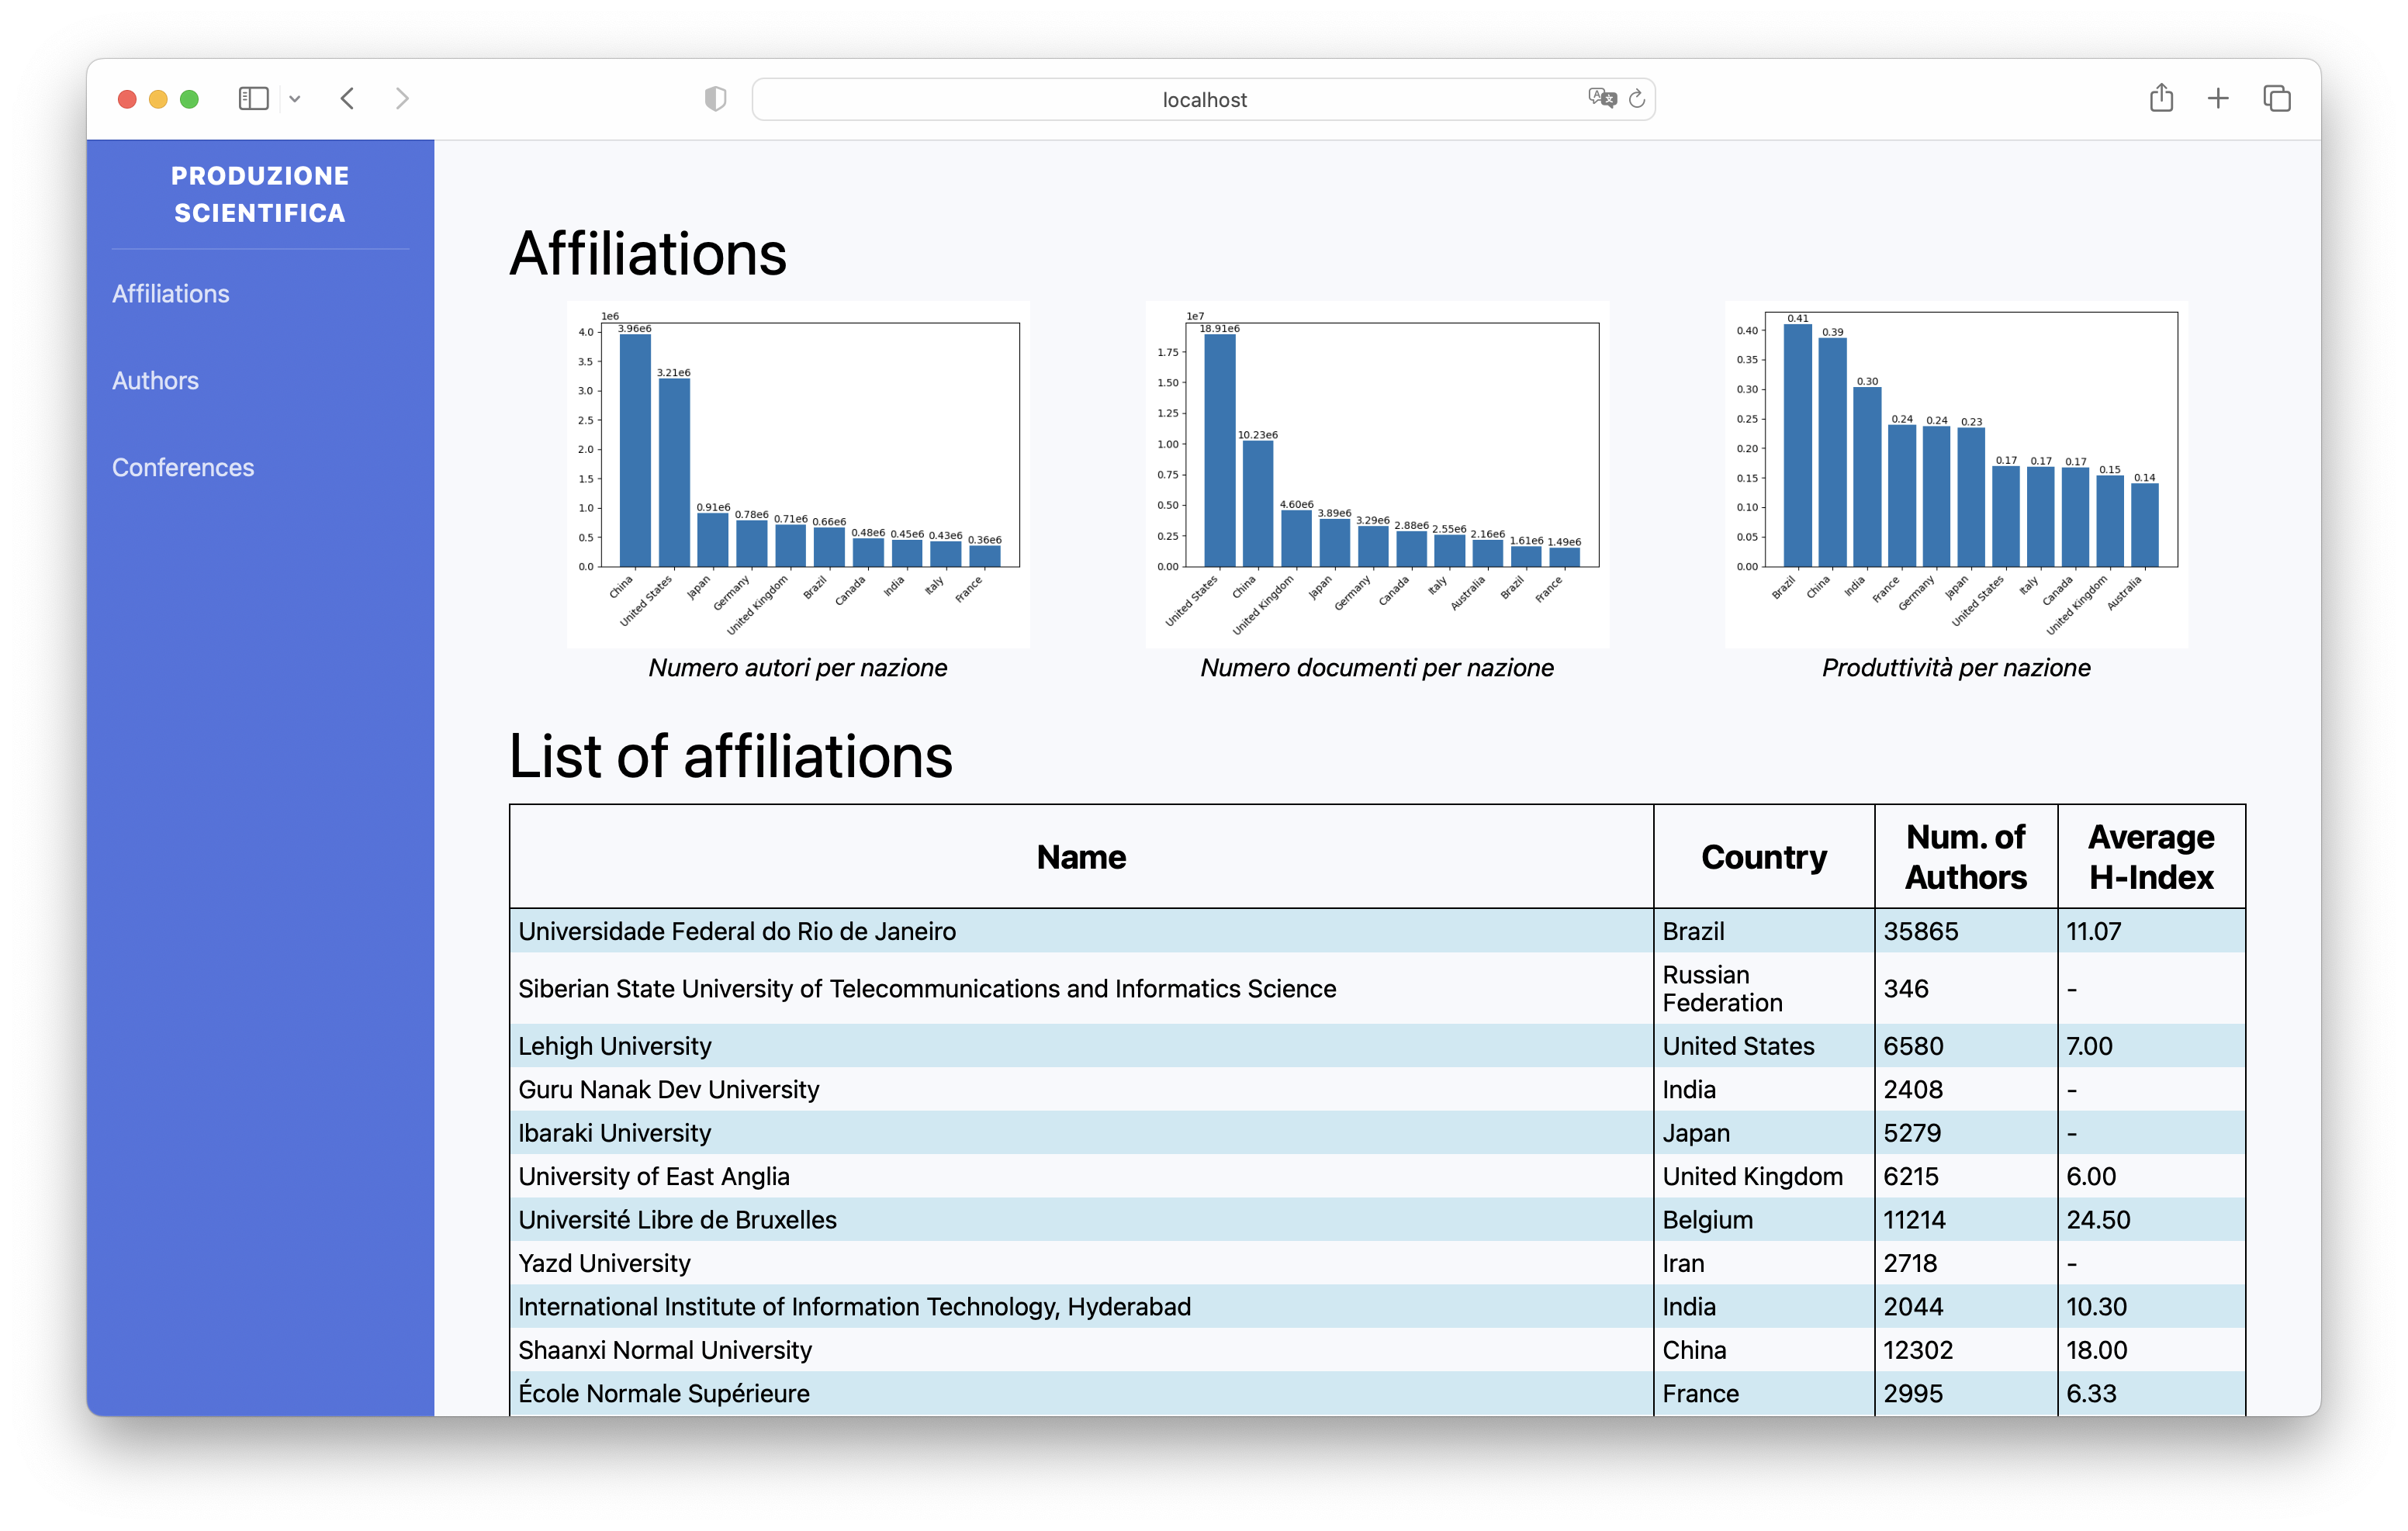
\includegraphics[width=0.8\linewidth]{affiliations.png}
  \caption{Pagina delle affiliazioni}
  \label{fig:affiliations}
\end{figure}

Nel Listing~\ref{lst:affiliation_html} è mostrato il codice per l'implementazione della pagina. 

\begin{lstlisting}[language=html, caption=Estratto di \texttt{template/affiliation.html}, label=lst:affiliation_html]



Affiliations - Produzione Scientifica



<div class="info">
  <div class="info-img">
    <img src="" />
    <span>Numero autori per nazione</span>
  </div>
  
  <div class="info-img">
    <img src="" />
    <span>Numero documenti per nazione</span>
  </div>
  
  <div class="info-img">
    <img src="" />
    <span>Produttivit&agrave; per nazione</span>
  </div>
  
</div>

<h1>List of affiliations</h1>

<table>
  <thead>
    <tr>
      <th>Name</th>
      <th>Country</th>
      <th>Num. of Authors</th>
      <th>Average H-Index</th>
    </tr>
  </thead>
  <tbody>
    
    <tr>
      <td>{{ a.name }}</td>
      <td>{{ a.country }}</td>
      <td>{{ a.author_count }}</td>
      <td>{{ h_index }}</td>
    </tr>
    
  </tbody>
</table>


\end{lstlisting}

\subsection{Calcolo delle metriche}

Le metriche sono calcolate tramite codice Python scritto ad-hoc per ogni
caso, usando i dati salvati nel database descritto nelle sezioni precedenti.
Per comodità ed organizzazione, per ogni metrica che ha una rappresentazione
tramite immagine è presente una view in \texttt{mainapp/images.py}.

Tali immagini sono ottenute tramite \texttt{matplotlib}. Dove necessario,
\texttt{pandas} e \texttt{numpy} offrono delle capacità di manipolazione dati
più avanzate di quanto disponibile direttamente dall'ORM di Django.

Come esempio, prendiamo la distribuzione delle conferenze usate in questo
progetto, analizzata ulteriormente in Sezione~\ref{sec:distrib-conferenze},
al fine di illustrare la realizzazione di una semplice immagine.
Come si può vedere nel Listing~\ref{lst:distrib-conf}, l'immagine viene creata
tramite una view di Django. La differenza principale è data dalla creazione
di una \texttt{figure.Figure} tramite la libreria \texttt{matplotlib}.
Inoltre, la risposta ritornata dalla view ha un \texttt{Content-Type} pari a
\texttt{image/png}, cosicché il client non interpreti erronamente il contenuto
come testo o come HTML.

\begin{lstlisting}[language=Python, caption=Distribuzione delle conferenze, label=lst:distrib-conf]
import matplotlib.figure as figure

def create_image(fig):
    resp = HttpResponse(content_type="image/png")
    fig.savefig(resp)
    return resp

def conferences_distribution(request):
    ratings = list(reversed(["A++", "A+", "A", "A-", "B", "B-"]))  # I want A++ on top
    counts = [len(Conference.objects.filter(ggs_rating=rating)) for rating in ratings]

    f = figure.Figure()
    ax = f.add_subplot()

    ax.barh(ratings, counts)

    return create_image(f)
\end{lstlisting}

Successivamente, come ogni altra view, è necessario fornire un URL a cui
Django risponderà con l'immagine creata. Tale passo è visibile nel
Listing~\ref{lst:distrib-conf-urls}, che contiene un estratto del file
\texttt{mainapp/urls.py}.

\begin{lstlisting}[language=Python, caption=Estratto di \texttt{mainapp/urls.py}, label=lst:distrib-conf-urls]
from django.urls import path
from . import views, images

urlpatterns = [
    # ...
    path(
        "conferences/distribution.png",
        images.conferences_distribution,
        name="conferences_distribution.png",
    ),
    # ...
]
\end{lstlisting}
